\begin{tikzpicture}[scale=0.36,rotate=90]
	
	\onslide<1->{
		\renewcommand{\forefillColor}{black!50!white}
		\renewcommand{\borderColor}{white}
		\renewcommand{\toprsidefillcolor}{red}
		\node(image)[scale=0.85,rotate=0] at (-4,-1.5){
			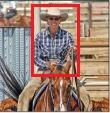
\includegraphics[scale=0.6]{images/cowboy_true.jpg}
		};
		\node[scale=0.85] at (-4,0-5.8){\tiny{Input}};
		
		\draw[->,line width=0.25mm](-2,-1.5)--(0,-1.5);

		\if 0	
		%% input layer
		\handmadecube{0}{4.5}{2.5}{-1}{0}
		\renewcommand{\toprsidefillcolor}{green}                  
		\handmadecube{0}{4.5}{2.5}{-1+0.2}{0}
		\renewcommand{\toprsidefillcolor}{blue!60!white}          
		\handmadecube{0}{4.5}{2.5}{-1+0.4}{0}
		\node[scale=0.85] at (1-0.6*2.6-0.1,0-4.8-0.5){\tiny{Input}};
		%     \node [scale=0.7, rotate=45] at (1-0.6*2.6+0.6,0.2) {\tiny{224}};
		%     \node [scale=0.7, rotate=90] at (1-0.6*2.6+0.2,-2) {\tiny{224}};
		\fi

		% Convolution Layer
		\renewcommand{\forefillColor}{red!50!white}
		\renewcommand{\borderColor}{white}
		\renewcommand{\toprsidefillcolor}{red!50!white!50}

		\pgfmathsetmacro{\seedx}{1}
		\pgfmathsetmacro{\seedy}{0}

		\foreach \xct/\yct in {1,...,2}
		{
			\pgfmathsetmacro{\xcti}{\seedx+\xct*0.1}
			\pgfmathsetmacro{\ycti}{\seedy}
			\handmadecube{0.5}{4.5}{2.5}{\xcti}{\ycti}
		}
		\node[scale=0.85] at (1+0.5,0-4.8){\tiny{Conv}};
		%     \node [scale=0.7, rotate=45] at (1-0.6*2.6+3.2,0.2) {\tiny{224}};
		%     \node [scale=0.7, rotate=90] at (1-0.6*2.6+0.2+2.6,-2) {\tiny{224}};
		%     \node[scale=0.7] at (1+0.725,0-4.2){\tiny{64}};
		
		
		
		% Pooling Layer
		\renewcommand{\forefillColor}{blue!50!white}
		\renewcommand{\borderColor}{white}
		\renewcommand{\toprsidefillcolor}{blue!50!white!50}
		
		\pgfmathsetmacro{\seedx}{2.5}
		\pgfmathsetmacro{\seedy}{0}

		\foreach \xct/\yct in {1}
		{
			%       \pgfmathsetmacro{\xcti}{\seedx+\xct*0.1}
			%       \pgfmathsetmacro{\ycti}{\seedy}
			
			\pgfmathsetmacro{\xcti}{\seedx+\xct*0.1}
			\pgfmathsetmacro{\ycti}{\seedy}
			\handmadecube{0.5}{3.8}{1.8}{\xcti}{\ycti}
		}
		\node[scale=0.85] at (0.5+2.8,0-4.2){\tiny{Max-pool}};
		%     \node [scale=0.6, rotate=45] at (1+3.7,0.2) {\tiny{112}};
		%     \node [scale=0.6, rotate=90] at (1+3.3,-2+0.5) {\tiny{112}};
		%     \node[scale=0.7] at (1+2.85,0-3.5){\tiny{64}};
		
		\foreach \xct in {1,2,3}
		{
			\filldraw[fill=gray!60](3+\xct,-1) circle(2pt) ;
		}

		\draw [thick,step=1,draw=blue!40!white](7,-3) rectangle (11,1);
		\draw [thin,step=0.5,draw=red!40!white](9.5,-0.5) grid (11,1);
		\draw [thin,step=0.5,draw=red!40!white](9.5,-0.5) -- (9.5,1);

		\filldraw[fill=green!50!white, draw=black,rounded corners] (13,4) rectangle (14,5);
		\draw [thin,step=1,draw=blue!40!white](7,-3) rectangle (11,1);
		\draw (13,-5) grid[xstep=1,ystep=1] (14,3);
		\node (x1) at (13.5,2.5) {\tiny{$x_1$}};
		\node (x2) at (13.5,1.5) {\tiny{$x_2$}};

		\foreach \y in {1,2,...,5}{
			\node (x2) at (13.5,1.5-\y) {\tiny{$\cdot$}};
		}

		\node (x2) at (13.5,-4.5) {\tiny{$x_{512}$}};
				
		\draw[->](11.1,-1)--(12.8,-1);
	}
	
	
	
\end{tikzpicture}